\begin{frame}{Stages of IPS}
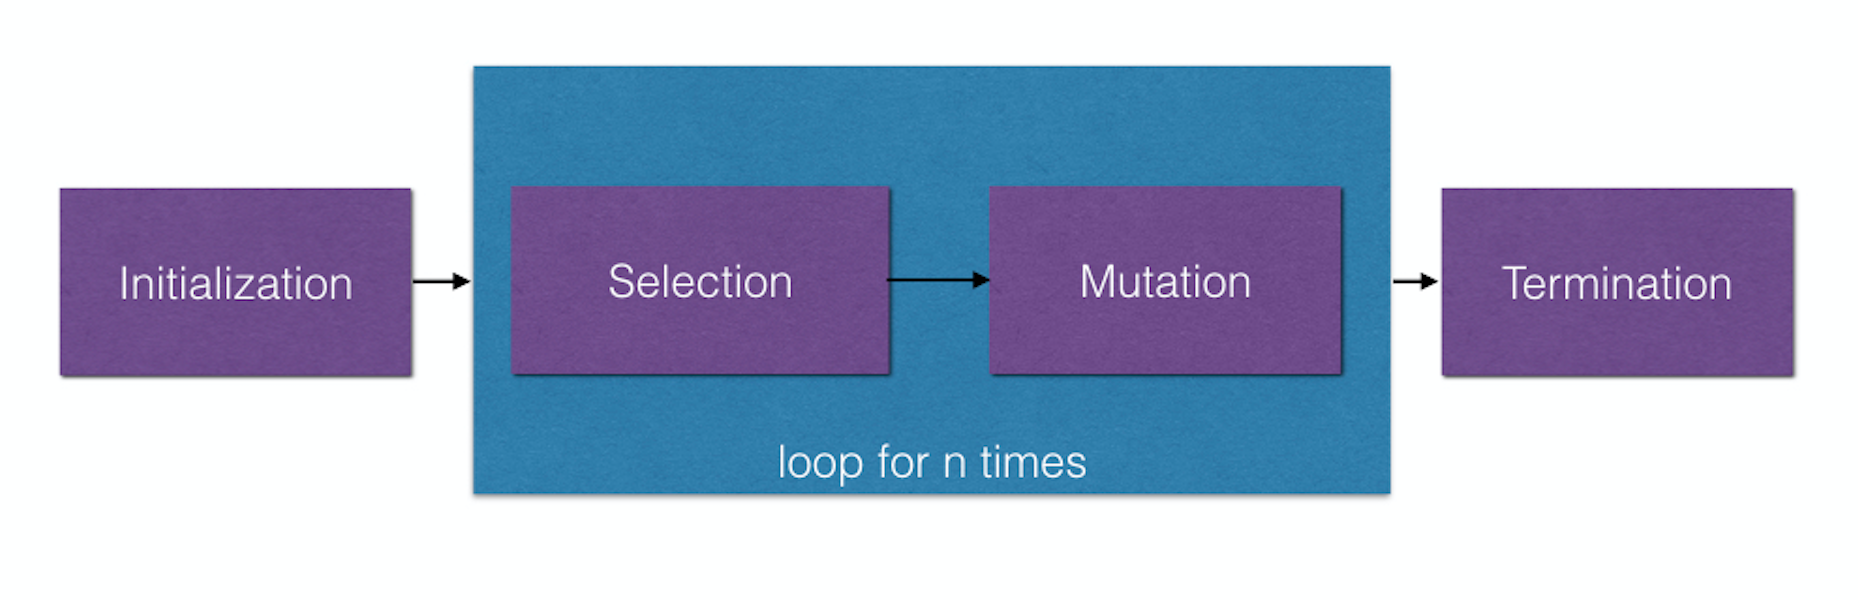
\includegraphics[width = \textwidth]{IPS_process}
\begin{itemize}
\item \textit{Initialization}: Initialize $M$ states $\left(t,L_{t}\right)$ and set up the parameters.
\item \textit{Selection}: Choose the states by resampling according weights of a potential function.
\item \textit{Mutation}: Evolve the system to the next state from the chosen states.
\item \textit{Termination}: Terminate after selecting and mutating for number of firms and estimate the probabilities
\end{itemize}
\end{frame}

\begin{frame}{Initialization}
	\begin{block}{Initial Value}
		\begin{equation*}
			\begin{split}
				\hat{X}_0^{(j)} &= \left( t_{0}^{(j)},L_{t_0}^{(j)} \right),  \quad 
				 1 \leq j\leq M                                                                    \\
			\end{split}
		\end{equation*}
	\end{block}
	\begin{itemize}
		\item  $ t_{0}^{(j)} = 0$ and $ L_{t_{0}}^{(j)} = 0$ $\forall 1 \leq j\leq M $ considering L as a pure birth process.
	\end{itemize}
\end{frame}

\begin{frame}{Selection}
	\begin{itemize}
		\item Sample independent $M$ particles with repetition from input $M$ paths according to empirical distribution under the given Gibbs measure.
		\item $\left(t^{(j)}_{n-1}, L_{t_{n-1}}^{(j)} \right)$ becomes $\left( \hat{t}_{n-1}^{(j)}, \hat{L}_{t_{n-1}}^{(j)}\right)$.
	\end{itemize}
	\begin{block}{Empirical distribution}
		\begin{equation*}
			\begin{split}
				\eta_{p}^{M}(dX) &= \frac{1}{M \hat{\eta}_{p}^{M}}\sum_{j=1}^{M}\left(\omega^{\alpha}(X_{p}^{(j)})\right) \times \delta_{{X}_p^{(j)}}(dX) \\
				&\text{Where} \quad
				\hat{\eta}_{p}^{M} = \mathbb{E}_{p}^{m}\omega^{\alpha}(X) =
				\frac{1}{M}\sum_{j=1}^{M}\left(\omega^{\alpha}(X_{p}^{(j)})\right)\\
				&\omega^{\alpha}(X)= 
                		\begin{cases}
    						\exp(\alpha),& \text{if } t < T\\
    						1,              & \text{otherwise}
						 \end{cases}
		    \end{split}
		\end{equation*}
	\end{block}
\end{frame}

\begin{frame}{Mutation}
	\begin{itemize}
		\item Evolve paths from $\left( \hat{t}_{n-1}^{(j)}, \hat{L}_{t_{n-1}}^{(j)}\right)$ to $\left(t^{(j)}_{n}, L_{t_{n}}^{(j)} \right)$.
		\item The function $\lambda$ is used to take each step until $t$ evolves to maturity time $T$. 
	\end{itemize}
	\begin{block}{Mutation Step}
		\begin{equation*}
				\begin{split}
					&t^{(j)}_{n}= \min\left(\hat{t}^{(j)}_{n-1} + \lambda\left(\hat{t}^{(j)}_{n-1},\hat{L}_{t_{n-1}}^{(j)}\right),T\right) \\
					& \lambda\left(\hat{X}\right) \sim \frac{1}{1-\frac{L_{t}}{N}} \times \exp(-x) \\
					&L_{t_{n}}^{(j)} = \hat{L}_{t_{n-1}}^{(j)} + 1 \text{ if } t^{(j)}_{n} 		\neq T					
				\end{split}	
		\end{equation*}
	\end{block}
\end{frame}

\begin{frame}{Termination}
	\begin{itemize}
		\item Teminate after running $n$ loops of mutation and selection. Here, $n =$ maximum number of defaults that can happen.
		\item Estimate default probability $p_k(T) = \mathbb{P}\left( L\left( T \right) = k
		      \right)$ using formula below.
	\end{itemize}
	\begin{block}{Estimation}
		\begin{equation*}
	\tilde{p}^m_{\ell}(T,\alpha) = \mathbb{E}^{m}_{n}{\delta_{\ell}(L(X))exp(-\alpha L(X))}\prod_{i=0}^{n-1}\mathbb{E}_{i}^{m}\omega^{\alpha}(X)
				\end{equation*}
			\end{block}
		\end{frame}
